\documentclass[no]{./../../common/SurferDesc}%%%%%%%%%%%%%%%%%%%%%%%%%%%%%%%%%%%%%%%%%%%%%%%%%%%%%%%%%%%%%%%%%%%%%%%
%
% The document starts here:
%
\begin{document}
\footnotesize
% Weltrekordfl�chen

%%% 1.Tafel

\begin{surferPage}
  \begin{surferTitle}En flate av sjuende grad med 99 singulariteter\end{surferTitle}   \\
  
	Oliver Labs konstruerte en flate av sjuende grad mens han jobbet med avhandlingen sin 
	ved Universitetet i Mainz i 2004. Dette er den forel�pige verdensrekorden for en flate av sjuende 
	grad, men det kan fortsatt finnes en slik flate med opptil $104$ singulariteter! Flaten til Labs har 
	symmetrien til et vanlig heptagon (bildet til venstre). Det blir synlig n�r vi ser p� flaten ovenfra (bildet til h�yre):
	
    \vspace*{-0.3em}
    \begin{center}
      \begin{tabular}{c@{\qquad}c}
        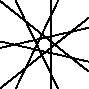
\includegraphics[height=1.5cm]{./../../common/images/labsseptic1.pdf}
        &
        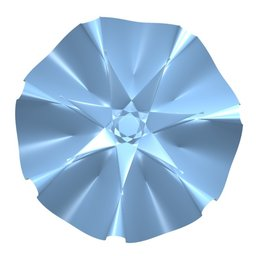
\includegraphics[height=1.5cm]{./../../common/images/labs_septic_von_oben}
      \end{tabular}
    \end{center}
    \vspace*{-0.3em}
	
	For � konstruere denne flaten, brukte Oliver Labs det algebraiske dataprogrammet {\sc Singular} 
	(Universitetet i Kaiserslautern). Det er velegnet til beregninger innen algebraisk geometri og singulariteter. 

	Labs brukte det faktum at man kan gj�re beregninger i endelige tallsystemer, som er systemer der tallene begynner 
	p� nytt n�r de kommer til enden. Vi kjenner til dette fra klokken; 24.00$=$0.00, 24.00 $+$ 1 time er ikke 25.00, men 1.00.
	

     
\end{surferPage}


\end{document}
%
% end of the document.
%
%%%%%%%%%%%%%%%%%%%%%%%%%%%%%%%%%%%%%%%%%%%%%%%%%%%%%%%%%%%%%%%%%%%%%%%
